\chapter{Literature Review}
% this chapter will be submitted to ATSIP This chapter reviews speech emotion
% recognition from bimodal information: acoustics and linguistics.  This
% section aims to outline the progress of research on speech emotion
% recognition recently. This outline includes emotion models, datasets,
% features and classifiers.  always ask why?!

This chapter reviews research on speech emotion recognition from two
modalities, acoustic and linguistic information. Four main components of speech
emotion recognition from multimodal fusion are described, including emotion
models; features; classifiers; and fusion methods. Each section after
Introduction describes each of these components with their advancements and
current limitations; the last section summarizes this chapter.

\section{Introduction}
% history of SER
Speech emotion recognition (SER) is a part of affective computing that relates
to, arises from, or influences emotions \cite{Picard} within speech. SER is an
attempt to make the computer to be able to recognize expressed emotion in a
given utterance. The earliest reported research on SER, perhaps, was the work
of Dellaert et al. \cite{Dellaert}. The study explores prosodic features with
several statistical pattern recognition techniques to classify the emotional
content of utterances. Under a limited number of data (1000 utterances), the
system achieved a comparable performance close to humans. 

% Why speech -- another milestone
Utilizing speech to identify humans' emotions rooted from the correlation
between voice and emotion. There is strong evidences that humans can recognize
other's emotions from their voices. In addition, given that speech is less
private than image and video, using speech to recognize emotion benefits future
implementation. Another milestone conducted by Petrushin \cite{Petrushin1998}
prove a pilot study to implement SER for call center application. This
laboratory-scale study, at that time, showed a potential application for SER
technologies.  Nowadays, this SER technology is ly available in the
commercial market, while its research is still ongoing. 

% SER dataset development (2000-2010)
The potential application of speech-based emotion recognition triggers the need
for such datasets. During 2000s, several datasets for emotion recognition
have been published, including the availability of speech data in the datasets.
Among many datasets, the following are commonly used in SER research: EmoDB
\cite{Burkhardt2005}, IEMOCAP \cite{Busso2008}, MSP-IMPROV \cite{busso2016msp},
and RAVDESS \cite{Livingstone2018}. The availability of these datasets
accelerates research on the SER area.

% SER in the modern era (2010-)
The progressive research on SER led to practical implementation in the
commercial industry. Nowadays, SER has been implemented in various
applications, both web/cloud-based applications or standalone applications.
Although it is useful to analyze the subject's affective state, these emerging
affective recognizer technologies have been criticized by others. Researchers
in psychology argued that due to individuals' high variability, the emotional
categories do not have an essence. The correlation between
particular facial expression and the corresponding basic emotion was not
strongly supported \cite{Barrett2019}. 

% Why fusing acoustic and linguistic: multimodal --> bimodal
Among many other issues, multimodal information fusion is a challenging task in
pattern recognition. Recent studies (e.g., \cite{Poria2017,Atmaja2020d,
Atmaja2020, Atmaja2019b}) confirm that multimodal classifiers outperform
unimodal classifiers. In SER itself, one of the main issues in searching for a
more predictive feature is whether it suffices to explore acoustic features
only, or it is necessary to combine acoustic features with other modalities
\cite{ElAyadi2011}. For speech, both acoustic and linguistic features can be
extracted. Thus, two pieces of information can be fused to evaluate the
effectiveness of information fusion from a single speech modality.

% why add text
The use of linguistic information for SER is also reasonable from an affective
computing point of view. In task-processing related tasks, linguistic
information is extracted from the text for sentiment analysis. This textual
information was also used to detect emotion in text
\cite{Alm2005,Mulcrone2012,Calvo2013}. In these works, textual information
showed encouraging results on both categorical and dimensional emotion
recognition from text. Fusing acoustic and linguistic information may improve
the performance of SER more significantly than other strategies.

% Shows bimodal results
Indeed, bimodal emotion recognition by fusing acoustic and linguistic
information shows significant performance improvement. References
\cite{Schuller2004,Schullera,Eyben2010,Ye2014,Tian2019} show the usefulness of
fusing acoustic and linguistic in different strategies to improve SER
performance. Different acoustic and linguistic features were fused using
different classifiers. Different fusing strategies were evaluated to
investigate the effectiveness of the fusion method.

% purpose of the chapter
This chapter aims to review current studies of bimodal emotion recognition by
utilizing acoustic and linguistic information. The scope of this study includes
the emotion models, features, classifiers, and fusion methods used in bimodal
SER. In the end of this chapter is a summary concluding this literature review.


% Although there are hundreds of research papers on speech emotion recognition,
% only 50s papers focused on bimodal emotion recognition by accommodating
% acoustic and linguistic information.

\section{Emotion models}
Before beginning to research emotion recognition, it is important to choose
which emotion model to adopt. According to \cite{Grandjean2008}, there are at
least three views to model humans' emotions: categorical emotion, dimensional
emotion, and componential appraisal emotion. However, all SER research employed
either first, second, or combination of both views as target emotion.  No
research was found on using speech data to obtain appraisal emotion. Thus, the
following description describes major models in active affective computing
research. 

\subsection{Categorical emotion}
Categorical emotion, also known as basic emotions, is the discrete emotion that
is independent of each other in its manifestations. Although the original idea
is to organize affective state into their emotion families (rather than
discrete emotion); however, most researchers agree that there are six basic
emotions: anger, fear, enjoyment, sadness, disgust, and surprise. The first
five emotions are backed by robust and consistent evidence, while the evidence
for the surprise is not as firm \cite{Ekman1992}. Nevertheless, these six basic
emotions have been a standard in categorical emotions.

Before Ekman coined the terms of basic emotions, Plutchik
\cite{plutchik1980emotion} have defined basic eights bipolar emotions: joy
(reproduction), sorrow/sadness (deprivation), acceptance/trust (incorporation),
disgust (rejection), surprise (orientation), anticipation (exploration), anger
(destruction), fear (protection). These eight emotions can be illustrated as a
wheel of emotion, as shown in Figure \ref{fig:plutchik_model}. Each emotion can
mix with other emotion to make up another emotion, as mixing colors. 

\begin{figure}[htbp]
    \centering
    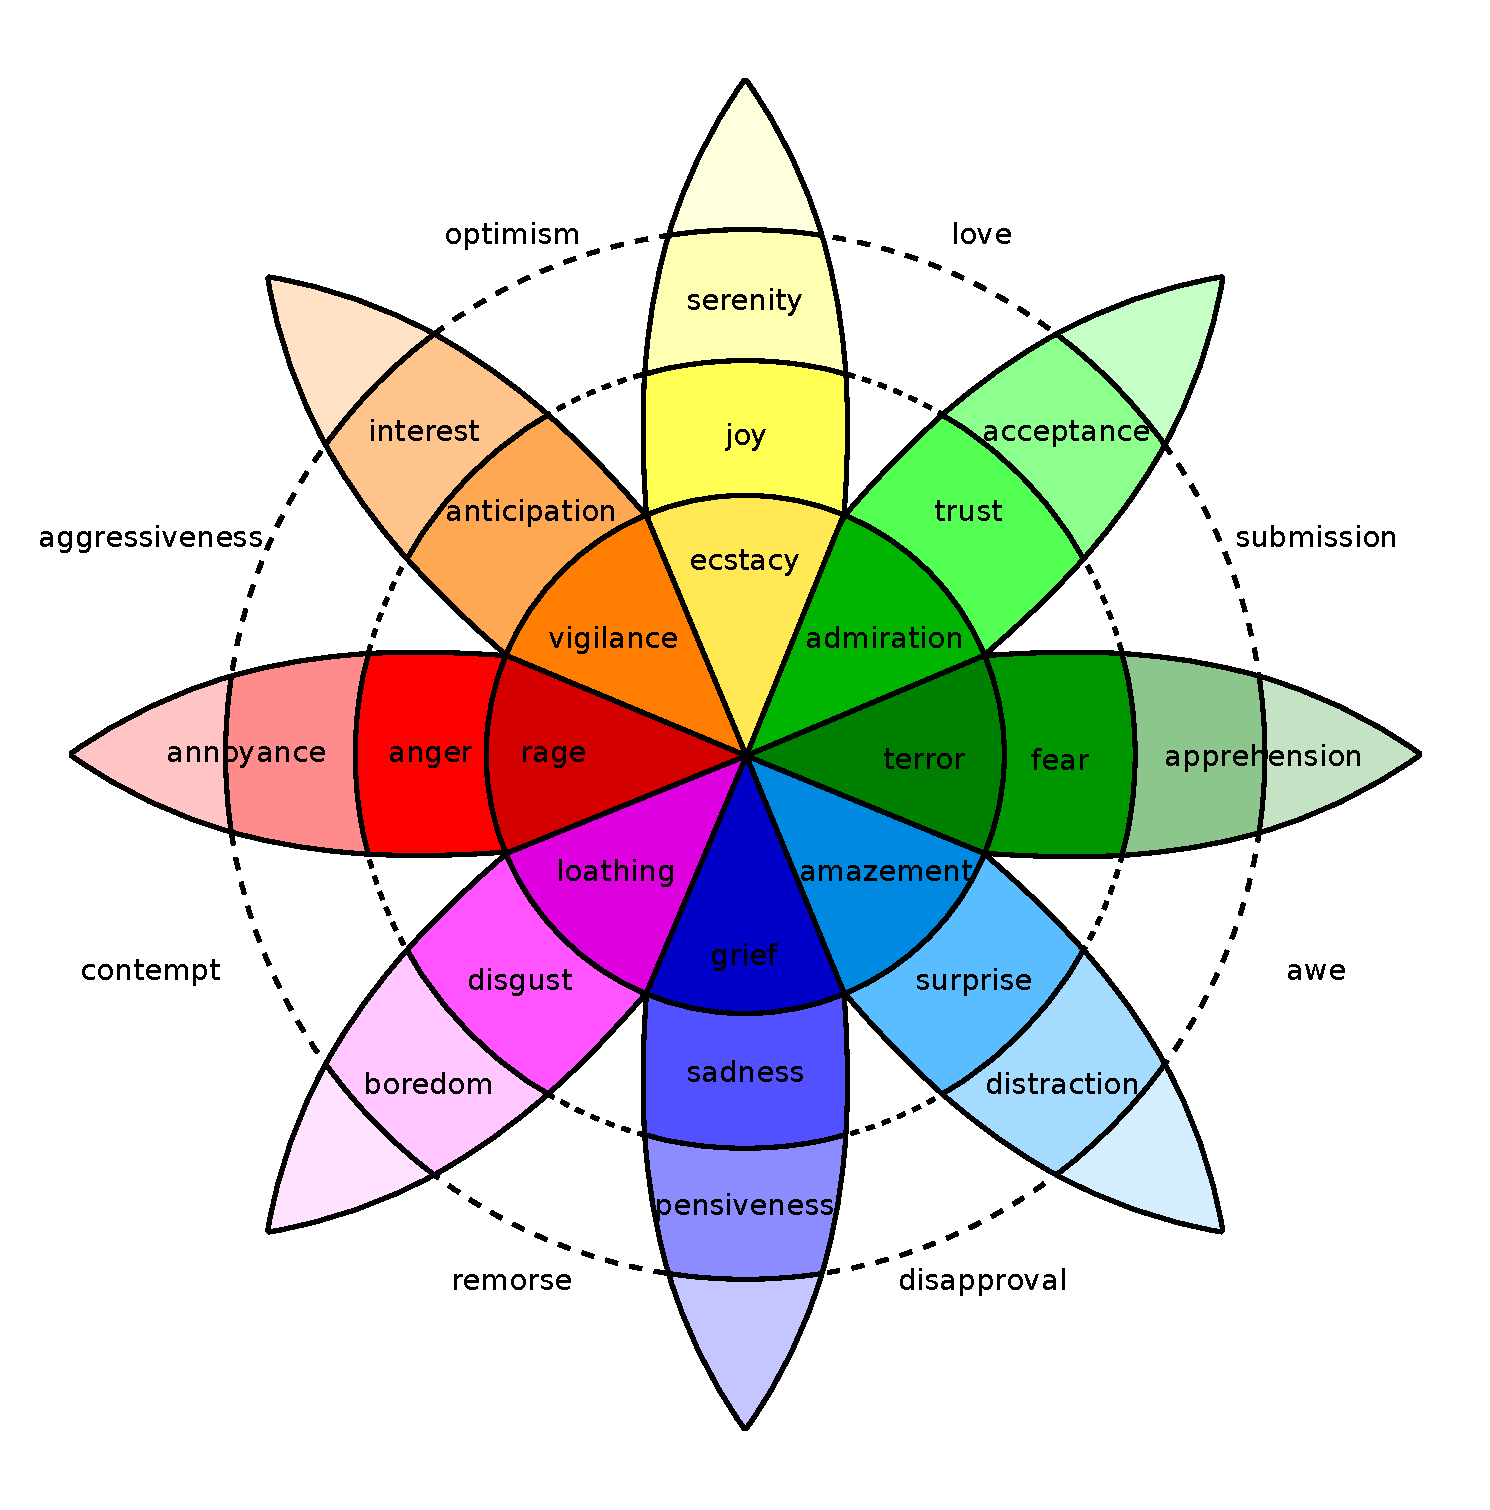
\includegraphics[width=4in]{../fig/plutchik_model.pdf}
    \caption{Plutchik wheel of emotions}
    \label{fig:plutchik_model}
\end{figure}

Instead of six, recent research suggests that four latent expressive patterns
were commonly observed in facial expressions \cite{Jack2016}. However, instead
of mentioning the name of basic emotions, the research utilized the term basic
"action unit pattern" (AU Pattern), from one to four. Although backed by
scientific evidence, this finding did not have any practical implementation
yet.

Ekman revised the characteristics which distinguish basic emotion from 9
criteria \cite{Ekman1992} to 11 criteria \cite{Ekman2005}. The new criteria
resulted in 15 emotions: amusement, anger, contempt, contentment, disgust,
embarrassment, excitement, fear, guilt, pride in achievement, relief,
sadness/distress, satisfaction, sensory pleasure, and shame. Du et al. 
\cite{Du2014} shows 21 categories of facial expressions by a facial action
coding system analysis. Furthermore, Cowen and Keltner \cite{Cowen2017} found
27 emotional experiences from facial expression by across self-report methods.
The growth of the number of categorical emotions, based on facial expression
measurement, confirms the high variability of humans expressed emotions. Darwin
argued that the biological category, including the emotion category, does not
have an essence; it is hard to map one-to-one facial expressions to emotional
states.

% closing statement for journal paper there is missing link from pyschological
% research to AI research. In psychologyical research unfound correlation
% between particular facial expression and related emotion. In contrast, AI
% research found that facial information is the richest modality to extract
% emotion from humans.  Most research on dividing emotion into categories were
% based on facial expression. Given inconsistency results, it is interesting to
% explore the possibility to find "fingerprint" of emotion in speech. In other
% words, what is the most important acoustic feature related to emotion?

% Most research conducted in SER were done from speech processing (engineering)
% point of view. It will be interesting to see results of psychoacoustics
% result of emotional speech (speech science). The investigation of particular
% emotion (e.g., anger) with its acoustic characteristics is a merit study.

\subsection{Dimensional emotion}
Instead of dividing emotion into several categories, a dimensional emotion
views emotion as continuous values/degrees of attributes in valence-arousal
space (VA) or valence-arousal-dominance (VAD) space. Valence is the degree of
positive or negative emotion, arousal refers to the level of activation from
sleepiness (low) to awakeness (high), and dominance is the degree of control
over the emotion \cite{Gunes2010}. In this theory, an emotion or affective
state is not independent of one to another. Rather, they are related one to
another in a systemic manner (in VA or VAD space). Russel argued that the
previous categorical emotion could be mapped within VA spaces. An illustration
of VA space with several emotion categories is shown in Figure
\ref{fig:va_space}.  


\begin{figure}[htbp]
    \centering
    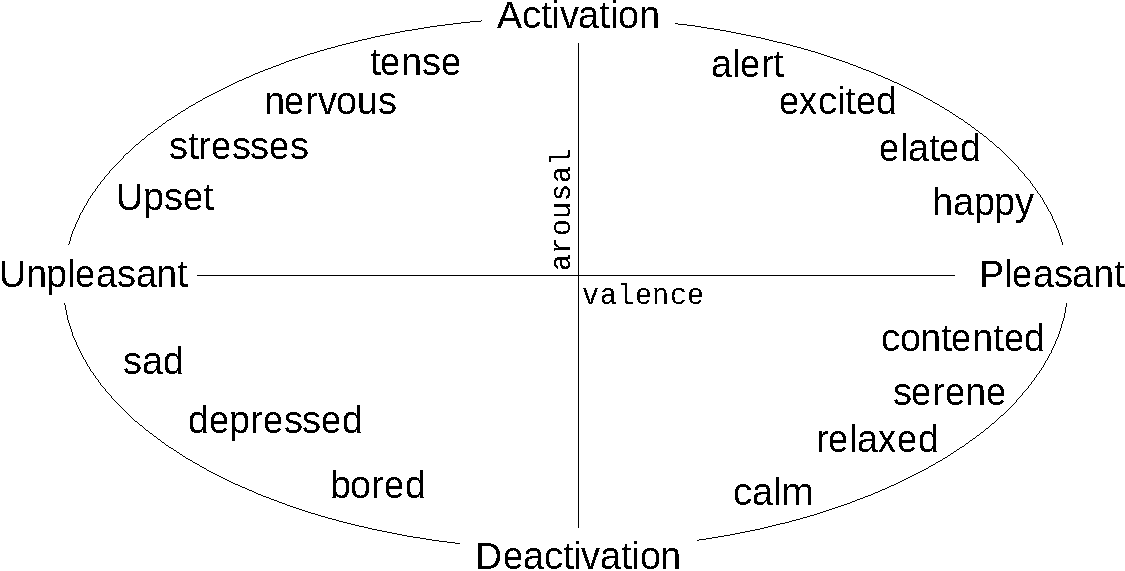
\includegraphics[width=.8\textwidth]{../fig/circumplex-crop.pdf}
\caption{Graphical representation of circumplex model (VA
space)\cite{Posner2005}; vertical axis: arousal; horizontal axis: valence}
    \label{fig:va_space}
\end{figure}

The search for higher dimensions for dimensional emotion is a worthwhile study.
Russel argued that all emotion categories could be mapped in 2D valence-arousal
space \cite{Russell1980a}. However, Fontaine et al. have found that the world
of dimensional emotion is not two or three dimensions, but four dimensions
\cite{Fontaine2017}. The fourth dimension is the unpredictability. In order of
importance, the order of dimensional emotions is valence, dominance, arousal,
and predictability. Fortunately, the similar fourth dimension is proposed in an
emotion recognition challenge \cite{Schuller2012}. In this challenge,
four-dimensional emotions were arousal, expectancy, power/dominance, and
valence. Expectancy, which represents the predictiveness of the subject's
feeling, is very similar to predictability/unpredictability in the previous
report.

The third emotion model, hybrid model or appraisal model, can be viewed as an
extension of the dimensional model. In this model, emotion categories are
spanned between bipolar dimensions. For instance, ``impatience" is located in
the upper part of the arousal axis (see \cite{Scherer2005}). This study of
appraisal-based emotion theory leads to the development of the Geneva emotion
wheel (GEW) rating study. This hybrid model has two similarities with the
previous 4D dimensional emotion model. First, the hybrid model also uses four
attributes (i.e., dimensions): valence, dominance/power, arousal, and
conducive/obstructive (instead of predictiveness). Second, in version 2.0 of
GEW, two axes used to draw emotion terms are valence and dominance/power, which
are the two most important emotional attributes according to
\cite{Fontaine2017}. Nevertheless, the use of the hybrid model in SER is not
familiar in the SER research community, perhaps due to these labels'
availability in the dataset.

\section{Features}
The input features to the SER system is the most important issue for developing
bimodal information SER. If the input is not informative for predicting emotion
or does not correlate to the predicted emotion, the prediction results will
suffer from low performance. In principle: garbage in, garbage out.  The
following divisions are useful features for SER from acoustics and linguistics.


\subsection{Acoustic features}
The correlation of acoustic features with emotion has been studied for many
years \cite{Scherer2005, Mairano}. The main division of acoustic features for
SER is the classical and modern approaches, i.e., hand-crafted features vs.
deep learning-based features. Hand-crafted features employed acoustic features
extracted per frame. These features often called local features or low-level
descriptor (LLD). On the other hand, statistical features computed from LLDs
are a new way to capture the dynamics among frames. This latter feature
extraction method is called global features, suprasegmental features,
high-level features, or high-level statistical function (HSF). Figure
\ref{fig:aco_feat} shows the division of acoustic features for SER.

\begin{figure}[htbp]
    \centering
    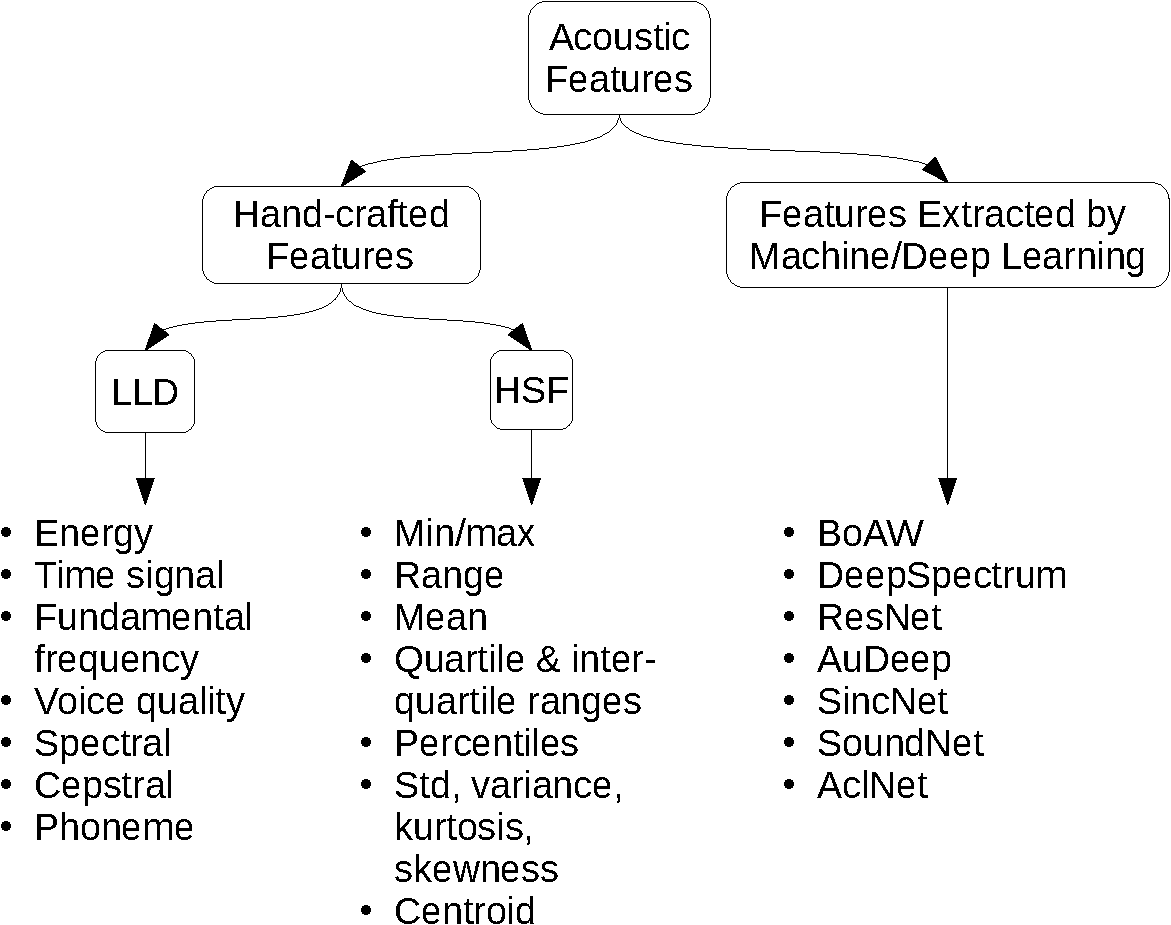
\includegraphics[width=.7\textwidth]{../fig/acoustic_features-crop.pdf}
    \caption{Division of acoustic features for SER}
    \label{fig:aco_feat}
\end{figure}

Eyben et al. \cite{Eyben2010} divided LLD and HSF into five groups: signal
energy, fundamental frequency (perception: pitch), voice quality, cepstral,
time signal, and spectral. Prosodic features ($f_o$, duration, intensity, voice
quality) have been known to have a strong correlation with emotion
\cite{Frick1985,Mozziconacci2002,Fritz2016} from a psychology point of view. In
acoustics, prosody is implemented into several acoustic features, including LLD
and HSF. Vayrynen \cite{Vayrynen2014} made a distinction between prosodic and
acoustic (non-prosodic) features. His study reported that a combination of
prosodic and acoustic features achieved comparable performance to human
reference on basic emotion recognition.

Both references \cite{Lee2002} and \cite{Schuller2004} employed $f_o$ and
energy-based acoustic features for SER. The former applied both LLD and HSF of
$f_o$ and energy features, while the latter only applied HSF of $f_o$ and energy
features. The latter reference found that $f_o$-based features correlated to
SER performance more than energy-based features.

As a `default' feature on most automatic speech recognition (ASR), MFCC has
been explored for SER. Metze et al. \cite{Metze2009} has found that MFCC is the
most informative acoustic features compared to other evaluate acoustic
features. Tripathi et al. \cite{Tripathi2019} found that MFCC performed better
than spectrogram features on unimodal acoustic SER. 

The shift from MFCC to mel-filterbank (MFB) features in ASR motivates SER
researchers to adopt a similar direction. Aldeneh et al. \cite{Aldeneh2017}
extracted 40 MFB features for dimensional SER tasks on the IEMOCAP dataset.
Zhang et al.  \cite{Zhang2019} employed a similar MFB with 40-dimensional with
z-normalization on categorical IEMOCAP and MSP-IMPROV datasets. Both research
showed fair performances (50\% -- 65\% accuracy) from MFB features for the SER
task.

Phoneme, the smallest unit of speech, has been investigated to be useful for
SER task. Zhang et al. \cite{Zhang2019} furthermore combined MFB with phoneme
for the same SER task. A combination of phoneme with MFB outperforms MFB-only
of phoneme-only input features. Yenigalla et al. \cite{Yenigalla2018} combined
phoneme embedding with a spectrogram. The phoneme embedding is generated from
the word2vec model \cite{Mikolov} and IEMOCAP speech data. The combination of
phoneme with spectrogram achieves the highest accuracy among individual
features.

Since most classifiers in modern SER systems used deep learning methods, it is
reasonable to extract an acoustic representation of speech in an end-to-end
manner via deep learning methods. In INTERSPEECH 2020 ComParE challenge, two
deep-learning-based features were given in the baseline system, DeepSpectrum
and AuDeep. The provided DeepSpectrum features with ResNet50 network achieve
the highest unweighted average recall (AUR) on the elderly emotion
sub-challenge test set.

\subsection{Linguistic features}
Linguistic features are the realization of linguistic information. It is also
called text features, textual features, lexical features, language features, or
semantic features. Although linguistic and lexical terms have different
meanings, i.e., language vs. word meaning,  these terms often used
interchangeably in computer science (or information processing). Text features
used in this study also have a different meaning from the same term used in
book or article writing. In book or article writing, the text features include
writing components such as a glossary, bold typeface, title, headings,
captions, and labels. In information science, text or linguistic features are
features extracted from written or spoken text.  Thus, the term linguistic
features is a preferable term than text features to avoid confusion among
readers.

% define a linguistic feature in general
Linguistics features used in emotion recognition represent numerical values
related to the emotional states in a word. The simplest way to build linguistic
features for emotion detection is by emotional keyword spotter
\cite{Chuang2004}. In this framework, every word is assumed to have a
correlation with emotion categories. For instance, the word ``disappointed''
can be represented as [(2, 0.2), (3, 0.6)] where 2 represents ``angry'' emotion
and 3 represent ``sadness'' emotion. Both 0.2 and 0.3 represent degrees of
emotion's intensity. This emotional keyword spotter can be expanded into an
emotional phrase spotter \cite{Schuller2004}.

The first systematic linguistic representation of a document, perhaps, is
TF-IDF (term-frequency inverse document frequency). TF is defined as the
frequency of a word in a particular document/utterance. IDF is defined as a
logarithm of the total number of documents' ratio to the total number
containing that word. TF-IDF is the multiplication of TF with IDF.

Bag-of-Words (BoW) is a numerical feature vector to represent ``words in a bag."
First, a fixed integer is assigned to each word occurring in any documents,
i.e., building a dictionary from a corpus by assigning a word to integer
indices.  Second, count the number of occurrences of each word and store it as
the value of feature $j$ where $j$ is the index of word $w$ in the dictionary
\cite{scikit-learn}.  These BoW features can be expanded for acoustic and
visual modalities (BoAW and BoVW).

Several lexicon dictionaries have been developed to inform the 'emotion score'
of emotional words. These dictionaries include DAL \cite{Whissell2009}, ANEW
\cite{Warriner2013}, VADER \cite{Hutto2014}, and NRC \cite{Mohammad2018}. Using
these dictionaries allows direct measurement of emotional words in the given
utterances. For instance, the word ``arose'' in DAL has values of 2.11, 2.00,
and 1.40 for pleasantness, activation, and imagery. These values are on a
3-point scale; different dictionaries have different scales.

The search for vector representation from a word led to the research of word
embedding or word vector. In this approach, a deep neural network (DNN) is used
to train a large corpus (i.e., a Wikipedia corpus) to generate word vectors
based on an algorithm. This approach has resulted in a new paradigm in the
vector representation of linguistic information of a word. Several models
exist, including word2vec, GloVe, FastText, and BERT. These models are detailed
in Chapter 5.

Figure \ref{fig:ling_feat} shows the division of linguistic features used in
SER task. Similar to acoustic features, there is a tendency to move to deep
learning-based features from hand-crafted features. The choice of linguistic
feature is usually based on the task as in other text processing areas.

% LSA is not mentioned yet
\begin{figure}[htbp]
    \centering
    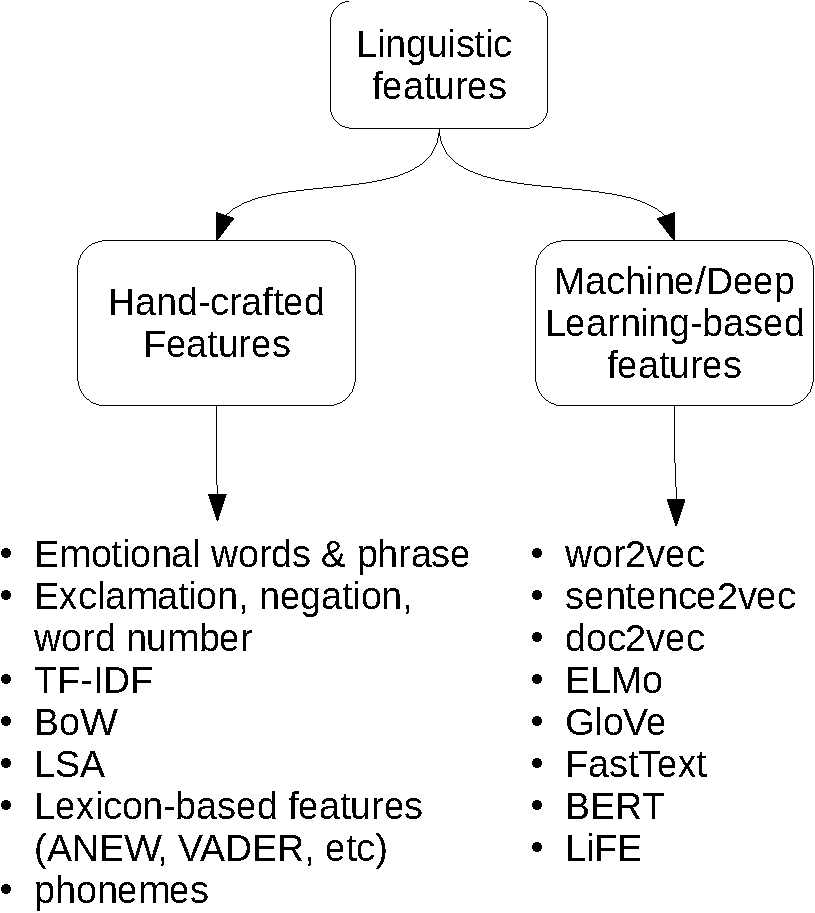
\includegraphics[width=0.6\textwidth]{../fig/linguistic_features-crop.pdf}
    \caption{Divisions of linguistic features used in SER}
    \label{fig:ling_feat}
\end{figure}

% division of linguistic features, list of linguistic features used in SER
% research

% closing statements in Acoustic, most features are hand-crafted features while
% in Linguistics, most features are extracted from deep learning

\section{Classifiers}
This section reviews the four most used classifiers in speech emotion
recognition.  One is a machine learning classifier, i.e., support vector
machine (SVM). Others are three deep learning classifiers, i.e., multilayer
perceptron (MLP), convolutional neural networks (CNN), and long short-term
memory (LSTM) neural networks. The brief descriptions of these classifiers are
given below.

\subsection{SVM}
SVM is a useful machine learning classifier for, generally, small datasets. For
categorical emotion recognition, SVM applies acoustic or linguistic features
for the given labels.  This SVM applied to the classification task is called
support vector classification (SVC).  For dimensional emotion recognition, SVM
applies regression analysis to map them to the given labels. This SVM for
regression task is called as support vector regression (SVR).

SVM can accept unimodal or multimodal inputs. In bimodal emotion recognition
from acoustic and linguistic information, SVM can be utilized in two-stage
scheme for evaluation of the emotion recognition system from DNNs outputs. In
bimodal information fusion, each prediction from the acoustic and text networks
is fed into the SVM.  From two values (e.g., valence predictions from the
acoustic and text networks), the SVM learns to generate a final predicted
degree (e.g., for valence). The concept of using the SVM as the final
classifier can be summarized as follows.

Suppose that two valence prediction outputs from the acoustic and text
networks, $x_i = [x_{ser}[i], x_{ter}[i]]$, are generated by the DNNs, and that
$y_i$ is the corresponding valence label. The problem in dimensional SER fusing
acoustic and text results is to minimize the following: 

\begin{equation}
\begin{aligned}
& \underset{w, b, \zeta, \zeta^*}{\text{min}}
& & \frac{1}{2} w^Tw + C \sum_{i=1}^n \zeta_i + C \sum_{i=1}^n \zeta_i^* \\
& \text{subject to}
& & w^T \phi (x_i)+b- y_i \leq \epsilon  + \zeta_i, \\
&&& y_i - w^T \phi (x_i) -b \leq \epsilon + \zeta_i^*, \\ 
&&& \zeta_i, \zeta_i^* \geq 0, i = 1, \ldots, n,
\end{aligned}
\end{equation}
where $w$ is a weighting vector, $C$ is a penalty parameter, $\zeta$ and
$\zeta^*$ is the distance between misclassified points and the corresponding
marginal boundary (above or below). Here, $\phi$ is the kernel function. On
the use for late fusion approach, the study choose a radial basis function
(RBF) kernel because of its flexibility to model a nonlinear process with a
dimensional emotion model close to this kernel. The function $\phi$ for the RBF
kernel is formulated as: 

\begin{equation}
 K(x_i, x_j) = e^{\gamma(x_i - x_j)^2},
 \label{tab:label}
\end{equation}
where $\gamma$ defines how much influence a single training has on the model.
All parameters in this SVM are obtained empirically via linear search in a
specific range. Although the explanation above uses valence, the same also
applies for arousal and dominance. 

% add literature review for SVM

\subsection{MLP}
MLP is a classical feedforward neural network by projecting input data into
linearly separable space using non-linear transformation. A hidden layer is an
intermediate layer between inputs and outputs, containing many perceptrons
(also called units or nodes). An MLP commonly refers to more than one hidden
layer. The MLP used here is similar to the definition of connectionist learning
proposed by Hinton \cite{Hinton1989}. A deeper layer MLP usually consists of
many layers to enable deep learning hierarchically. This neural network
architecture is also known as dense network or fully-connected (FC) network.
  
% parameter
MLP is a simple yet powerful tool for combining acoustic and linguistic
information via network concatenation. Mathematically, the combined
acoustic+linguistic network could be formulated as in equation \ref{eq:mlp}.
Here, $f(y)$ denotes the output of the corresponding layer; $W_1, W_2$ denote
the weights from previous layers ($a$: acoustic; $l$: linguistic), i.e., a dense
layer after LSTM for each network, and the current hidden layer, respectively;
$x_a$ and $x_l$ are the acoustic features and word embeddings, respectively;
$b$ is a bias; and $g$ is an activation function. Thus, the output of the that
dense layer is 
\begin{equation}
f(y) = W_2 g ([W_{1a}^\top xa + b_{1a};W_{1l}^\top xl + b_{1l}]) + b_2
\label{eq:mlp}.
\end{equation}

Schuller et al. \cite{Schuller2004} utilized MLP for combining acoustic and
linguistic information. Their evaluation using MLP showed lower error than the
fusion method by means of logical ``OR''. Callejas and L\'opez-C\'ozar
\cite{Callejas2008} compared baseline majority-class method to MLP for
evaluating the effect of context information on categorical SER task. The
result shows that MLP outperforms the baseline method in six out of eight
scenarios. Zhang et al.  \cite{Zhang2019} used MLP in all experiments involving
acoustic features, phoneme, and combination of both; MLP showed its
effectiveness on both single-stage and multi-stage SER tasks.

% add literature review for MLP

\subsection{CNN}
% review cnn here, take the theory from d2l.ai, refer to CNN in SER paper.
CNN is a class of neural networks that contain a convolutional layer.
Convolution is a mathematical operation between two functions by measuring the
overlap of both when one function (``input'') is flipped and shifted by another
function (``kernel''). The resulting output, which is the goal of a convolution
layer, is a feature map. This convolution operation is similar to
cross-correlation; cross-correlation does not flip the second function.
Convolution is also can be seen as cross-correlation with a scalar bias. In
deep learning literature, the convolution terminology views cross-correlation
as convolution since many deep learning frameworks did not take bias into
account by default. 

The convolutional network is often applied to image-like data. Time-series
data, including acoustic feature vector, can be fed into convolutional networks
using 1-dimensional (1D) CNN. To take the most benefit of CNN, spectrogram and
mel-filterbank (MFB) features are frequently used to input the SER system. For
text processing, the main idea for CNN is to compute vectors for n-gram (e.g.,
2-, 3-, and 4-gram) and group them afterward. CNN is commonly used for both
speech and language processing. 

Apart from convolutional layers, CNN typically still needs a fully-connected
layer (FC or MLP). The feature map as the output of the convolution layer is
fed into MLP to obtain desired outputs. Although recently it is found
unnecessary \cite{Springenberg2015}, a CNN commonly uses pooling layers after
convolutional layers for mitigating and reducing spatial representation
\cite{Zhang2020}.

Yenigalla et al. \cite{Yenigalla2018} experimented with CNN for categorical
SER by inputting phoneme, spectrogram, and combination of both. The combination
of both phoneme embeddings and spectrogram achieved the highest performance.
The architecture of each phoneme and spectrogram networks was convolution layer
and max-pooling and FC layer. Both networks are concatenated by FC layers
to obtain the outputs.

Instead of phoneme and spectrogram, Huang et al. \cite{Huang2018} proposed to
use bag-of-audio-words for the input of the CNN-based SER system. The
architecture was similar to \cite{Yenigalla2018}, i.e., convolution, pooling,
and FC layer.  The result shows that the use of BoAW outperforms raw acoustic
features.

Cho et al. \cite{Cho2018} combined acoustic and linguistic information for
categorical SER; the acoustic inputs used an LSTM network while the linguistic
inputs used a multi-resolution CNN. A multi-resolution CNN is utilized to
emotion words by employing word embedding, convolution layer, and global mean
pooling. The combination of acoustic network with LSTM, linguistic network with
CNN, and emotion vector (e-vector) achieved the highest performance compared to
unimodal results.

While most bimodal SER research used CNN for linguistic and LSTM for acoustic
information processing, Sebastian and Pierucci \cite{Sebastian2019}, used LSTM
for text and CNN for speech. The CNN architecture contains two convolution
layers and two FC layers. In this case, the performance of CNN-based text
emotion recognition is the lowest among other models.


Cai et al. \cite{Cai2019} replaced FC layers in most CNN architectures with
bidirectional LSTM with attention. The improved architecture was called
CNN-Bi-LSTM-Attention (CBLA). On both unimodal and multimodal, CBLA outperforms
MLP models by considering both global and temporal information in the data.

\subsection{LSTM}
Long Short-Term Memory (LSTM) neural networks is an extension of a recurrent
neural network. The idea of using LSTM networks comes from an approach that
human has the persistence to keep memory long in a short-term period. Humans do
not start their thinking from scratch every second. When reading a paper, a
reader understands each word based on the understanding of the previous words.
Humans do not throw everything away and start thinking from scratch again. The
thoughts have persistence.

Three gates are introduced in LSTMs: the input gate ($\mathbf{I}_t$), the
forgetting gate ($\mathbf{F}_t$), and the output gate ($\mathbf{G}_t$). In
addition to that we introduce memory cells that take the same shape as the
hidden state.  A memory cell is just a fancy version of a hidden state, custom
engineered to record additional information. The three gates in LSTM are
defined as:

\begin{align}
\mathbf{I}_t &= \sigma(\mathbf{X}_t \mathbf{W}_{xi} + \mathbf{H}_{t-1} \mathbf{W}_{hi} + \mathbf{b}_i),\\
\mathbf{F}_t &= \sigma(\mathbf{X}_t \mathbf{W}_{xf} + \mathbf{H}_{t-1} \mathbf{W}_{hf} + \mathbf{b}_f),\\
\mathbf{O}_t &= \sigma(\mathbf{X}_t \mathbf{W}_{xo} + \mathbf{H}_{t-1} \mathbf{W}_{ho} + \mathbf{b}_o).
\end{align}

Then the candidate memory cell, memory cell, and hidden state are calculated on
the following equations:

\begin{align}
\widetilde{C}_t &= \text{tanh}(\mathbf{X}_t \mathbf{W}_{xc} + \mathbf{H}_{t-1} \mathbf{W}_{hc} + \mathbf{b}_c), \\
\mathbf{C}_t &= \mathbf{F}_t \odot \mathbf{C}_{t-1} + \mathbf{I}_t \odot \tilde{\mathbf{C}}_t, \\
\mathbf{H}_t &= \mathbf{O}_t \odot \tanh(\mathbf{C}_t).
\end{align}

Graphical illustration of LSTM explained by equations above is shown in Figure
\ref{fig:lstm}.

\begin{figure}[!hb]
\centering
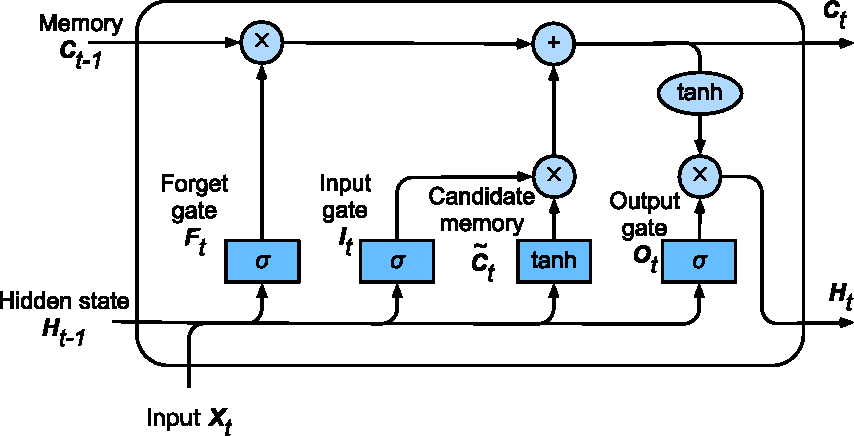
\includegraphics[width=4.5in]{../fig/lstm_3.pdf}
\caption{Graphical illustration of LSTM \cite{Zhang2020}}
\label{fig:lstm}
\end{figure}

% add literature review for LSTM
LSTM has dominated the classifiers used in both ASR and SER. Since the data
(i.e., input features) are sequence, a recurrent neural network is a
straightforward way to process these data. In addition, LSTM is able to model
long-range context in emotional features to map it with the emotional labels.
Tian et al. \cite{Tian2015} used the LSTM classifier to build hierarchical
neural networks. In \cite{Cho2018}, LSTM was used to train acoustic features
before the network was concatenated with a CNN-based linguistic network.

Instead of unidirectional LSTM, bidirectional LSTM (BLSTM) has been utilized to
learn information both from the past and the future inside the network
(unidirectional LSTM only learns from the past). In \cite{Cai2019}, BLSTM is
used for the textual network rather than the acoustic network. This
bidirectional LSTM is often combined with an attention model to boost the
performance of the SER task \cite{Atmaja2019}. However, using BLSTM doubles the
model's complexity, making the model may be not suitable for real-time
applications.

\section{Fusion Methods} 
Multimodal fusion in technology is the combination of information that comes
from different sources \cite{Khaleghi2013}. This terminology is similar but
different to the human multimodal perception. In human multimodal perception,
the information comes from different sensory organs; in technology, this
requirement is not necessary.  Multimodal fusion can be viewed as multisensor
data fusion. In this terminology, the `sensor' is the soft sensor. Acoustic and
linguistic feature extractors can be regarded as soft sensors in bimodal
acoustic-linguistic information fusion.

Fusing acoustic and linguistic features have been attempted at the early stage
of speech emotion recognition research. The first work on fusing acoustic with
linguistic information has been performed by Lee et al. \cite{Lee2002} by
combining acoustic and language features at the decision level using logical
``OR''. If at least one decision corresponds to a specific emotion, then the
result is this specific emotion. This earliest work only involved negative and
non-negative emotion categories.

Fusing acoustic and linguistic information for SER can be accomplished in
several ways, Figure \ref{fig:ser_bimodal} shows the classification. Early
fusion combines acoustic and linguistic information at the feature level; late
fusion combines results from acoustic and linguistic information at the
decision level.  Early fusion, furthermore, can be split into three main
categories: feature concatenation, networks/model concatenation, and
hierarchical model.  Hierarchical model, as proposed in
\cite{Majumder2018,Tian2019}, can be regarded as early fusion since the method
fuses features at a different level of layers, not at the decision level.

\begin{figure}[htbp]
    \centering
    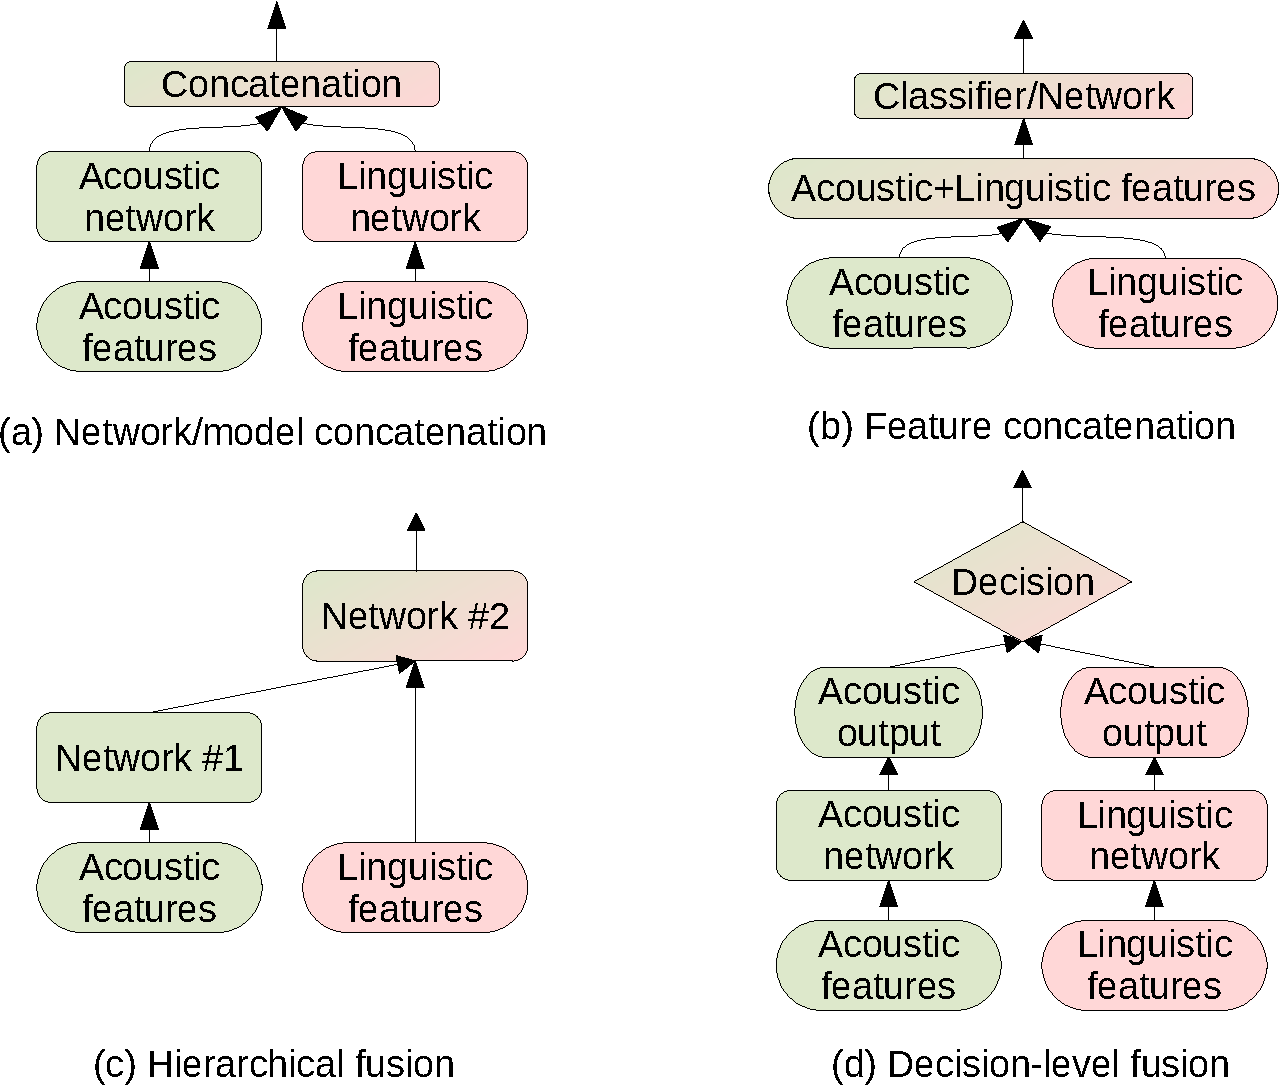
\includegraphics[width=0.9\textwidth]{../fig/ser_bimodal-crop.pdf}
    \caption{Different scheme of fusing acoustic with linguistic information; (a), (b), (c): early fusion approach; (d): late fusion approach}
    \label{fig:ser_bimodal}
\end{figure}

Eyben et al. \cite{Eyben2010} proposed an online method to detect not only
valence and arousal but also the time when those emotion attributes are
detected. They used a recurrent neural network (RNN) based on long short-term
memory (LSTM) to recognize a framewise valence-arousal continuum with time. By
adding a keyword spotter, they were able to improve the performance by using
regression analysis. The results were measured in Pearson correlation
coefficient (PCC).  They also found that keywords like ``again,'' ``angry,''
``assertive,'' and ``very'' were related to activation, while typical keywords
correlated to valence were ``good,'' ``great,'' ``lovely,'' and ``totally.''
Similar to that idea, Karadogan and Larsen \cite{Karadogan2012} used affective
words from Affective Norms for English Words (ANEW) to determine
valence-arousal values and combine them with a result from acoustic features.
The latter paper also obtained similar improvements over any single
modality.

Ye and Fan \cite{Ye2014} used bimodal features from acoustic and text
information to recognize emotion within speech. The acoustic features were
trained in two parallel classifiers: an SVM and a backpropagation network. The
text features were trained in two serial classifiers, which were both Naive
Bayes classifiers.  The second classifier acted as a filter for unreliable
parts from the first classifier. Decision-level fusion (late fusion) was then
implemented by combining the acoustic and text features with tree-weighting
factors for the SVM, backpropagation network, and text classifiers. The
resulting fusion method obtained 93\% accuracy, as compared to 83\% from the
acoustic features only and 89\% from the text features only. The task was
categorical emotion detection from a Chinese database. Similar to that approach
for a categorical task, Jin et al. \cite{Jin2015} used the IEMOCAP dataset to
test combinations of acoustic and text features for SER. The novelty of their
method was the use of an emotion vector for lexical features, which improved
the accuracy in four-class emotion recognition from 53.5\% (acoustic) and
57.4\% (text) to 69.2\% (acoustic + linguistic).

Aldeneh et al. \cite{Aldeneh2017} used acoustic and lexical features to detect
the degree of valence from speech. They used 40 mel-filterbanks (MFBs) as
acoustic features and word vectors as linguistic features. Continuous valence
values were then converted to three categorical classes: negative, neutral, and
positive. Using that approach, they improved the weighted accuracy from 64.5\%
(linguistic) and 58.9\% (acoustic) to 69.2\% (acoustic + linguistic). 

Yoon et al. \cite{Yoon2018} used audio and text networks to predict emotion
classes from the IEMOCAP dataset. Both networks used RNNs with inputs of
mel-frequency cepstral coefficients (MFCCs) for audio and word vectors for
text. The proposed multimodal dual recurrent encoder (MDRE) improved on the
single-modality RNNs from 54.6\% (audio) and 63.5\% (text) to 71.8\% (audio +
text). Atmaja et al.  \cite{Atmaja2019b} obtained a better result by using 34
acoustic features after silence removal and combining them with word
embeddings. With  LSTM used for the text and dense networks for speech, the
latter paper obtained an accuracy of 75.49\% on the same dataset and task
(categorical emotion recognition).

Instead of using lexical features, Zhang et al. \cite{Zhang2019} used phonemes
and combined them with acoustic features to recognize valence in speech. They
used 39 unique phonemes from the IEMOCAP and MSP-IMPROV datasets and a
40-dimensional log-scale MFB energy for the acoustic features. Using a scaled
version of valence, converted from a 5-point scale to three categorical
classes, they showed that their multistage fusion model outperformed all other
models on both IEMOCAP and MSP-IMPROV.

\section{Summary}
This chapter reviews research on bimodal speech emotion recognition from
acoustic and linguistic information. The study focuses on four building blocks
of SER from bimodal information: emotion models, features, classifiers, and
fusion methods.  There are three emotion models developed in psychological
research; however, most SER research focused on the categorical model. There is
a move to extract acoustic features in the feature extraction step by using
deep-learning methods, while deep-learning-based linguistic features already
dominated text processing research, including SER from linguistic information.
Four common classifiers for SER are briefly described.  Although more advanced
DNN architectures have been developed, bimodal SER still relies heavily on SVM,
MLP, CNN, and LSTM architectures. Finally, the fusion of different information
can be performed in several methods; these methods can be divided into early
and late fusions. While this literature study presents the current state of
speech emotion recognition research in these four blocks, the raised issues in
SER research will be highlighted in the next Research Methodology chapter along
with other related sections. 
